%% Ein einfaches Template für einen Übungsbericht unter Verwendung des Hagenberg
%% Setups, basierend auf der LaTeX 'report' Standardklasse.
%%% äöüÄÖÜß  <-- keine deutschen Umlaute hier? UTF-faehigen Editor verwenden!

%%% Magic Comments zum Setzen der korrekten Parameter in kompatiblen IDEs
% !TeX encoding = utf8
% !TeX program = pdflatex
% !TeX spellcheck = de_DE
% !BIB program = biber

\documentclass[german,notitlepage,smartquotes]{hgbreport}
% Zulässige Optionen in [..]:
%    Hauptsprache: 'german' (default), 'english'
%    Option zur Umwandlung in typografische Anführungszeichen: 'smartquotes'
%    APA Zitierstil: 'apa'
%    Erzeuge keine separate Titelseite: 'notitlepage'
%%%-----------------------------------------------------------------------------

\RequirePackage[utf8]{inputenc} % bei Verw. von lualatex oder xelatex entfernen!

\renewcommand{\chapter}[1]{} % Deaktiviere den \chapter Befehl
\graphicspath{{images/}}     % Verzeichnis mit Bildern und Grafiken
\bibliography{references}    % Biblatex-Literaturdatei (references.bib)
\ExecuteBibliographyOptions{backref=false} % Keine Rückreferenzen bei Quellen

%%%-----------------------------------------------------------------------------
\setcounter{chapter}{2}	% <----- Auf die Übungsnummer setzen
%%%-----------------------------------------------------------------------------

\author{Julian Jany}                        % Name
\title{GP2 Generative Programmierung -- SS 2022\\ % Name der Übung
				Übungsabgabe \arabic{chapter}}
\date{\today}

%%%-----------------------------------------------------------------------------
\begin{document}
%%%-----------------------------------------------------------------------------
\maketitle
%%%-----------------------------------------------------------------------------

% \renewcommand{\abstractname}{Anmerkungen}
% \begin{abstract}\noindent
% \ldots
% \end{abstract}

%%%-----------------------------------------------------------------------------
\lstset{language=C++,
		basicstyle=\ttfamily\footnotesize,
		keywordstyle=\color{blue}\ttfamily,
		stringstyle=\color{red}\ttfamily,
		commentstyle=\color{green}\ttfamily,
		morecomment=[l][\color{magenta}]{\#}
}
%%%-----------------------------------------------------------------------------


\section{JSON Validator}

\subsection{Lösungsidee}

Die JSON Grammatik Beschreibung auf \url{https://www.json.org} wurde in die entsprechende Notation von \texttt{Boost.Spirit} transformiert.
Da nur Parsing ohne semantische Aktionen gefordert war und "Edge-cases" ignoriert werden konnten, war die Implementierung unkompliziert.

\subsection{Code}

\lstinputlisting[caption=Json.h, language={[11]C++}]{src/JsonValidator/Json.h}
\lstinputlisting[caption=main.cpp, language={[11]C++}]{src/JsonValidator/main.cpp}

\clearpage

\subsection{Test}

\begin{figure}[h]
\centering
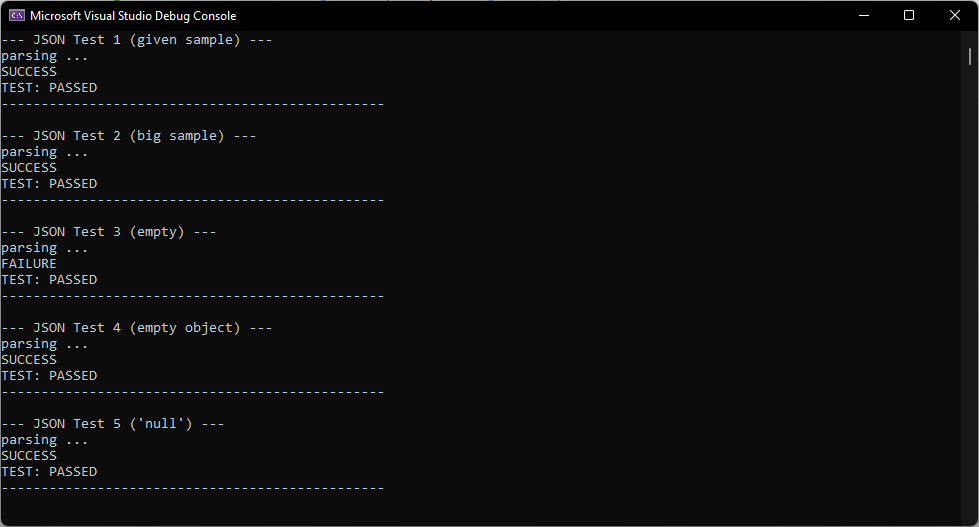
\includegraphics[width=.95\textwidth]{json_test}
\caption{Testausgabe der JsonValidator-Tests}
\label{fig:json_test}
\end{figure}

\clearpage

%%%-----------------------------------------------------------------------------

\section{Mini-LOLCODE with Boost.Spirit}

\subsection{Lösungsidee}

\subsubsection{Consolen-Ausgabe}

Die korrekte Ausgabe von Zeilenumbrüchen wurde so umgesetzt, dass anstelle eines optionalen "!"-Literals eine Regel "! oder eps" verwendet wurde. So kann der Epsilon-Ausdruck mit der sematischen Aktion \texttt{print\_newline()} versehen werden.

\subsubsection{Kommentare}

Zum Überspringen von Kommentaren im Quellcode werden, wie es \texttt{Boost.Spirit} vorsieht, sogenannte \texttt{Skipper} eingesetzt. Dadurch kann im Prinzip eine kleine Grammatik zur Beschreibung der Kommentare verwendet werden.

\subsubsection{Variablen}

Variablen werden in einer \texttt{map} verwaltet und von ihrem Bezeichner auf den Wert abgebildet. Sie können mit den entsprechenden sematischen Aktionen geschrieben (\texttt{set\_\-var\-iable()}) und "gelesen" (\texttt{print\_variable()}) werden.

\subsubsection{Arithmetische und Boolsche Operationen}

Implementiert wurden alle einfachen arithmetischen Operationen resp. Summe, Differenz, Produkt und Quotient. Die implementierten boolschen Operationen sind Und, Oder, exklusiv-Oder und Negation.
Dabei wurde immer nach dem selben Schema vorgegangen. Der erste Ausdruck der Operation wird dem Rückgabeparameter der Regel zugewiesen, anschließend wird der zweite Ausdruck mit diesem verknüpft und der Rückgabeparameter überschrieben.


\subsection{Code}

\lstinputlisting[caption=LOLCode.h, language={[11]C++}]{src/LOLCode/LOLCode.h}
\lstinputlisting[caption=main.cpp, language={[11]C++}]{src/LOLCode/main.cpp}

\clearpage

\subsection{Test}

\begin{figure}[h]
\centering
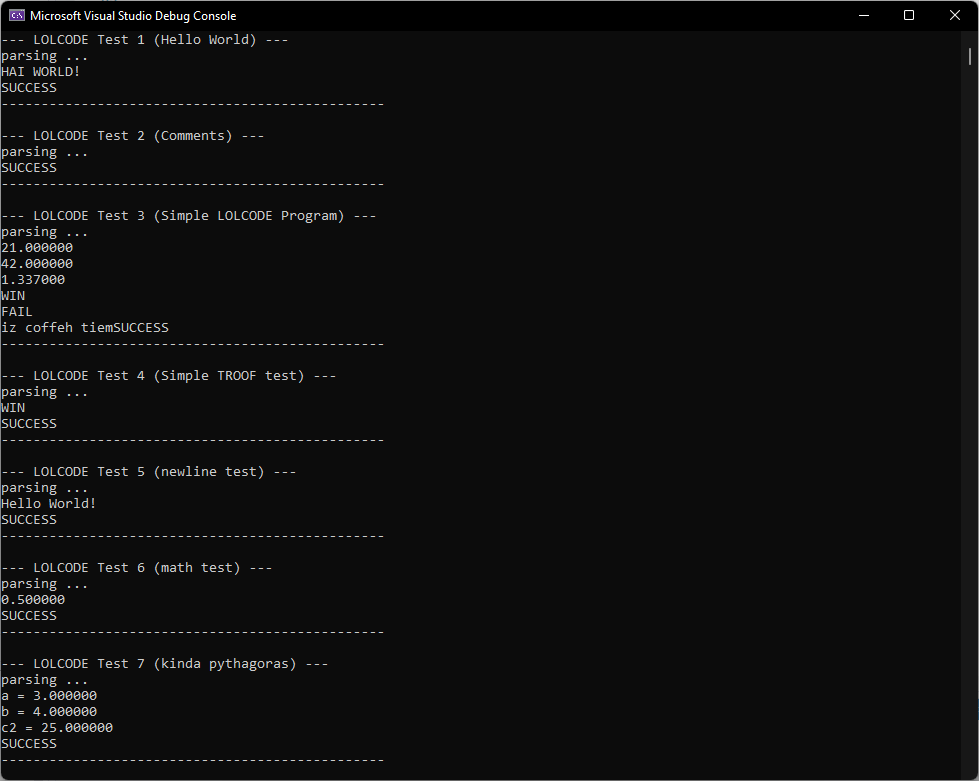
\includegraphics[width=.95\textwidth]{lolcode_test}
\caption{Testausgabe der LOLCode-Tests}
\label{fig:lolcode_test}
\end{figure}

%%%-----------------------------------------------------------------------------

%\section*{Zusammenfassung und Anmerkungen}

%%%-----------------------------------------------------------------------------

% \section*{Quellen}

% \printbibliography[heading=noheader]

%%%-----------------------------------------------------------------------------
\end{document}
%%%-----------------------------------------------------------------------------